\subsubsection{Simulations: dataset dimensions}
\vspace{1.5cm}
\begin{table}[H]
\centering
\begin{tabular}{l|l|rrrrrr}
\multicolumn{2}{l|}{} & \multicolumn{1}{c}{SpiecEasi} & \multicolumn{1}{c}{gCoda} & \multicolumn{1}{c}{ecoCopula} & \multicolumn{1}{c}{MRFcov} & \multicolumn{1}{c}{MInt} & \multicolumn{1}{c}{EMtree} \\ 
\hline
\multirow{3}{*}{{\rotatebox[origin=c]{90}{Easy}}} 
    & Cluster & 0.86  (0.20) & 0  (0.08) & 0.33  (0.14) & 0.27 (0.13) & 0.38  (0.17) & 0.12  (0.09) \\ 
    & Erdös   & 0.86  (0.21) & 0  (0.15) & 0.29  (0.15) &0.25 (0.14)& 0.38  (0.15) & 0.12  (0.08) \\ 
    & Scale-free & 0.82 (0.15) & 0.84 (0.07) & 0.85 (0.02) & 0.8 (0.03) & 0.85 (0.04) & 0.19 (0.11)  \\  \hline
\multirow{3}{*}{{\rotatebox[origin=c]{90}{Hard}}} & Cluster  & 0.88 (0.12) & 0 (0.2) & 0.15 (0.18) & 0.27 (0.19) & 0.77 (0.09) & 0.39 (0.09) \\ 
 & Erdös.     & 0.88 (0.11) & 0 (0.24) & 0 (0.15) & 0.32 (0.2) & 0.77 (0.1) & 0.39 (0.09) \\ 
 & Scale-free &0.83 (0.1) & 0.88 (0.05) & 0.86 (0.02) & 0.8 (0.03) & 0.85 (0.04) & 0.33 (0.09)  \\ \hline
\end{tabular}
\caption{Medians and standard-deviation of FDR computed on 100 graphs of each type (\textit{easy}: $n=100, p=20$, \textit{hard}: $n=50, p=30$)}
\label{medFDR}
\end{table}

\begin{table}[ht]
\centering
\begin{tabular}{l|l|rrrrrr}
\multicolumn{2}{l|}{} & \multicolumn{1}{c}{SpiecEasi} & \multicolumn{1}{c}{gCoda} & \multicolumn{1}{c}{ecoCopula} & \multicolumn{1}{c}{MRFcov} & \multicolumn{1}{c}{MInt} & \multicolumn{1}{c}{EMtree} \\ \hline
\multirow{3}{*}{{\rotatebox[origin=c]{90}{Easy}}} &Cluster &0.16 (0.11) & 0.05 (0.07) & 1.04 (0.48) & 0.62 (0.25) & 0.3 (0.13) & 0.81 (0.17) \\ 
& Erdös &0.15 (0.09) & 0.06 (0.08) & 0.95 (0.5) & 0.57 (0.26) & 0.3 (0.14) & 0.65 (0.12) \\ 
 & Scale-free & 0.42 (0.17) & 1.97 (0.82) & 6.05 (0.4) & 4.11 (0.34) & 2(0.54) & 1.05 (0.1) \\ \hline
\multirow{3}{*}{{\rotatebox[origin=c]{90}{Hard}}}  & Cluster &  0.21 (0.08) & 0.02 (0.03) & 0.02 (0.17) & 0.15 (0.09) & 0.68 (0.3) & 0.49 (0.11)  \\ 
 & Erdös & 0.21 (0.08) & 0.02 (0.02) & 0 (0.18) & 0.15 (0.08) & 0.66 (0.25) & 0.52 (0.1)  \\ 
 & Scale-free &  0.55 (0.12) & 2.16 (0.88) & 6.14 (0.47) & 3.38 (0.29) & 1.86 (0.32) & 1.03 (0.09)  \\ 
   \hline
\end{tabular}

\caption{Medians and standard-deviation of density ratio computed on 100 graphs of each type (\textit{easy}: $n=100, p=20$, \textit{hard}: $n=50, p=30$)}
\label{meddens}
\end{table}

\begin{table}[ht]
\centering
\begin{tabular}{l|l|rrrrrr}
\multicolumn{2}{l|}{} & \multicolumn{1}{c}{SpiecEasi} & \multicolumn{1}{c}{gCoda} & \multicolumn{1}{c}{ecoCopula} & \multicolumn{1}{c}{MRFcov} & \multicolumn{1}{c}{MInt} & \multicolumn{1}{c}{EMtree} \\ \hline
\multirow{3}{*}{{\rotatebox[origin=c]{90}{Easy}}} & Cluster & 1.77 & 13.89 & 1.74 & 0 & 0 & 0 \\
 & Erdös &0.68 & 11.95 & 0.99 & 0 & 0.83 & 0  \\
 & Scale-free & 0 & 0 & 0 & 0 & 0 & 0\\ \hline
\multirow{3}{*}{{\rotatebox[origin=c]{90}{Hard}}} & Cluster &  0 & 14.05 & 23.40 & 0 & 0 & 0\\
 & Erdös &0 & 20.85 & 27.28 & 0.60 & 0 & 0  \\
 & Scale-free &  0 & 0.43 & 0 & 0 & 0 & 0  \\ \hline
\end{tabular}
\caption{Percentage of empty networks computed on 100 graphs of each type (\textit{easy}: $n=100, p=20$, \textit{hard}: $n=50, p=30$)}
\label{empty}
\end{table}

%\newpage
\begin{table}[ht]
\centering
\begin{tabular}{l|l|rrrrrr}
   n & Criteria (\%) & SpiecEasi & gCoda & ecoCopula & MRFcov & MInt & EMtree \\ 
  \hline
\multirow{3}{*}{{$100$}} & FDR& 0.93(0.04) & 0(0.04) & 0.33(0.11) & 0.29(0.08) & 0.85(0.04) & 0.41(0.08) \\ 
  & density ratio & 0.62(0.13) & 0.08(0.07) & 0.92(0.3) & 0.56(0.14) & 1.97(0.54) & 1.08(0.08) \\ 
  & empty graphs & 0 & 1.88 & 0 & 0 & 0 & 0 \\  \hline
 \multirow{3}{*}{{$50$}} & FDR & 0.94(0.05) & 0(0.13) & 0(0.16) & 0.33(0.16) & 0.85(0.04) & 0.62(0.06) \\ 
 & density ratio & 0.61(0.13) & 0.04(0.03) & 0.08(0.24) & 0.22(0.1) & 1.86(0.32) & 1.14(0.11) \\  
  & empty graphs & 0& 5.97 & 15.46 & 0 & 0 & 0 \\  \hline
\end{tabular}
\caption{Medians and standard-deviation of FDR and density ratio critera, as well as percentage of empty networks computed on 100 scale-free graphs with $p=50$ nodes and $n=100$ or $n=50$ samples.}
\label{perfSF50}
\end{table}

\begin{table}[ht]
\centering
\begin{tabular}{ll|rrrrrr}
 
n & p & SpiecEasi & gCoda & ecoCopula & MRFcov & MInt & EMtree \\ 
  \hline
  100 & 20 & 15.92(0.05) & 0.34(0.79) & 4.84(0.24) & 5.62(0.79) & 66.83(36.03) & 5.06(0.74) \\    
  50 & 30   & 16.3(0.06) & 21.93(32.44) & 11.27(0.84) & 5.97(1.45) & 73.73(31.57) & 3.71(1.11) \\   \hline
  100 & 50 & 20.48(1.4) & 1.07(0.24) & 24.99(0.32) & 15.53(0.12) & 50.51(28.52) & 20.54(2.42) \\   
  50 & 50   & 20.01(2.76) & 44.21(14.78) & 32.75(1.39) & 27.32(1.8) & 55.96(23.26) & 11.54(0.66) \\ \hline
\end{tabular}
\caption{Median and standard-deviation of running times in seconds  of methods for the inference of scale-free structures with different values of the number of samples $n$ and of the number of species $p$. }
\label{timeSF}
\end{table}

\vspace{1.5cm}

\begin{figure}[H]
    \centering
    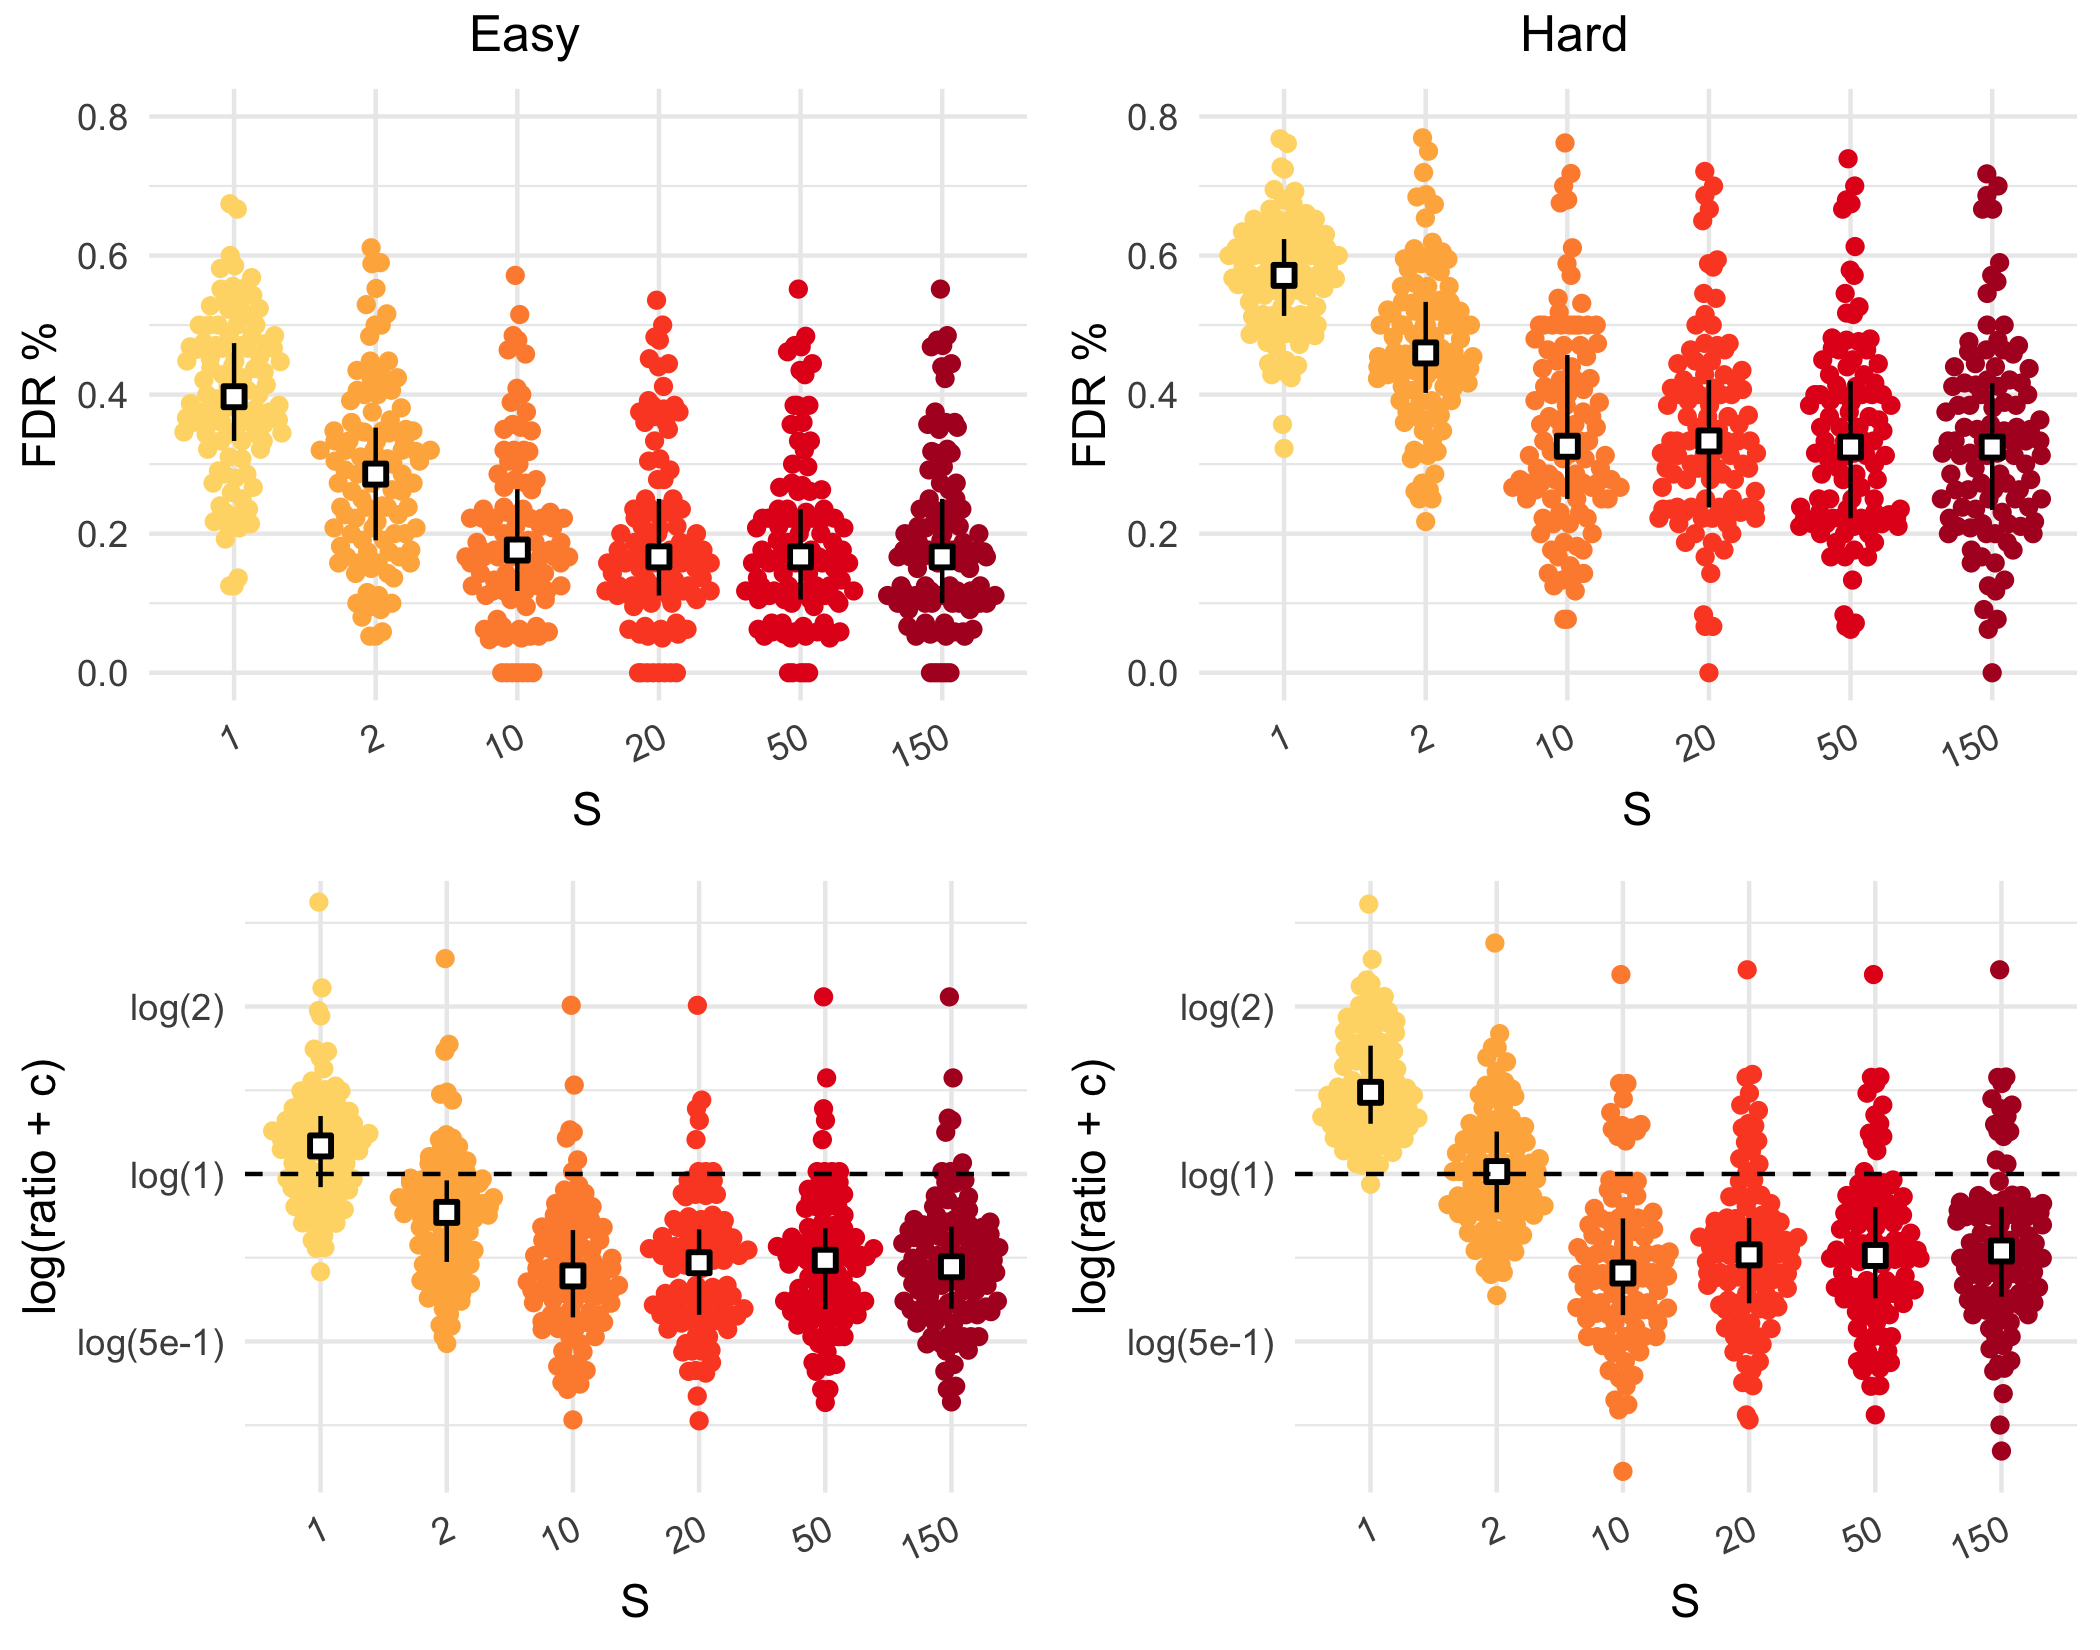
\includegraphics[width=10cm]{figs/S_effect.png}
    \caption{FDR and density ratio measures of EMtree with varying values of number of sub-samples $S$ (Erdös structure).}
    \label{Seffect}
\end{figure}


\begin{table}[ht]
\centering
\begin{tabular}{l|rrrrrr}
  $S$ & \multicolumn{1}{c}{1} & \multicolumn{1}{c}{2} & \multicolumn{1}{c}{10} & \multicolumn{1}{c}{20} & \multicolumn{1}{c}{50} & \multicolumn{1}{c}{150} \\ \hline
  Easy & 0.66  (0.15) & 1.86  (0.23) & 7.00  (0.81) & 12.29  (1.27) & 29.50  (3.39) & 87.30  (10.36) \\ 
  Hard & 0.45  (0.12) & 1.44  (0.14) & 5.06  (0.78) & 8.97  (0.87) & 23.35  (2.40) & 69.29  (10.83) \\ 
   \hline
\end{tabular}
\caption{Median and standard-deviation running-time values in seconds of EMtree with different values of the number of sub-samples $S$ for the inference of Erdös structures.}
\label{timesS}
\end{table}

\subsubsection{Simulations: network density}

\begin{table}[H]
\centering
\begin{tabular}{l|rr|rr}
    & \multicolumn{1}{c}{$n < 50$} & \multicolumn{1}{c}{$n\geq 50$} & \multicolumn{1}{c}{$p < 20$} & \multicolumn{1}{c}{$p\geq 20$} \\  \hline
  EMtree    &   0.41 (0.11)	&   0.60 (0.15) &   0.38 (0.12) &    0.71 (0.21)      \\ 
  gCoda     &   0.12 (0.47)	&   0.07 (0.03) &   0.05 (0.03) &    0.09 (0.06)     \\ 
  SpiecEasi &   2.41 (0.25)	&   2.41 (0.25) &   2.39 (0.25) &    2.42 (0.25)      \\ 
   \hline
\end{tabular}
\caption{Median and standard-deviation of running times for each method in seconds, for $n$ and $p$ parameters. corresponding to Erdös and cluster structures with $5/p$ densities.}
\label{timeDenser}
\end{table}
 
\subsubsection{Illustrations: edge frequency threshold}

\begin{figure}[H]
    \centering
    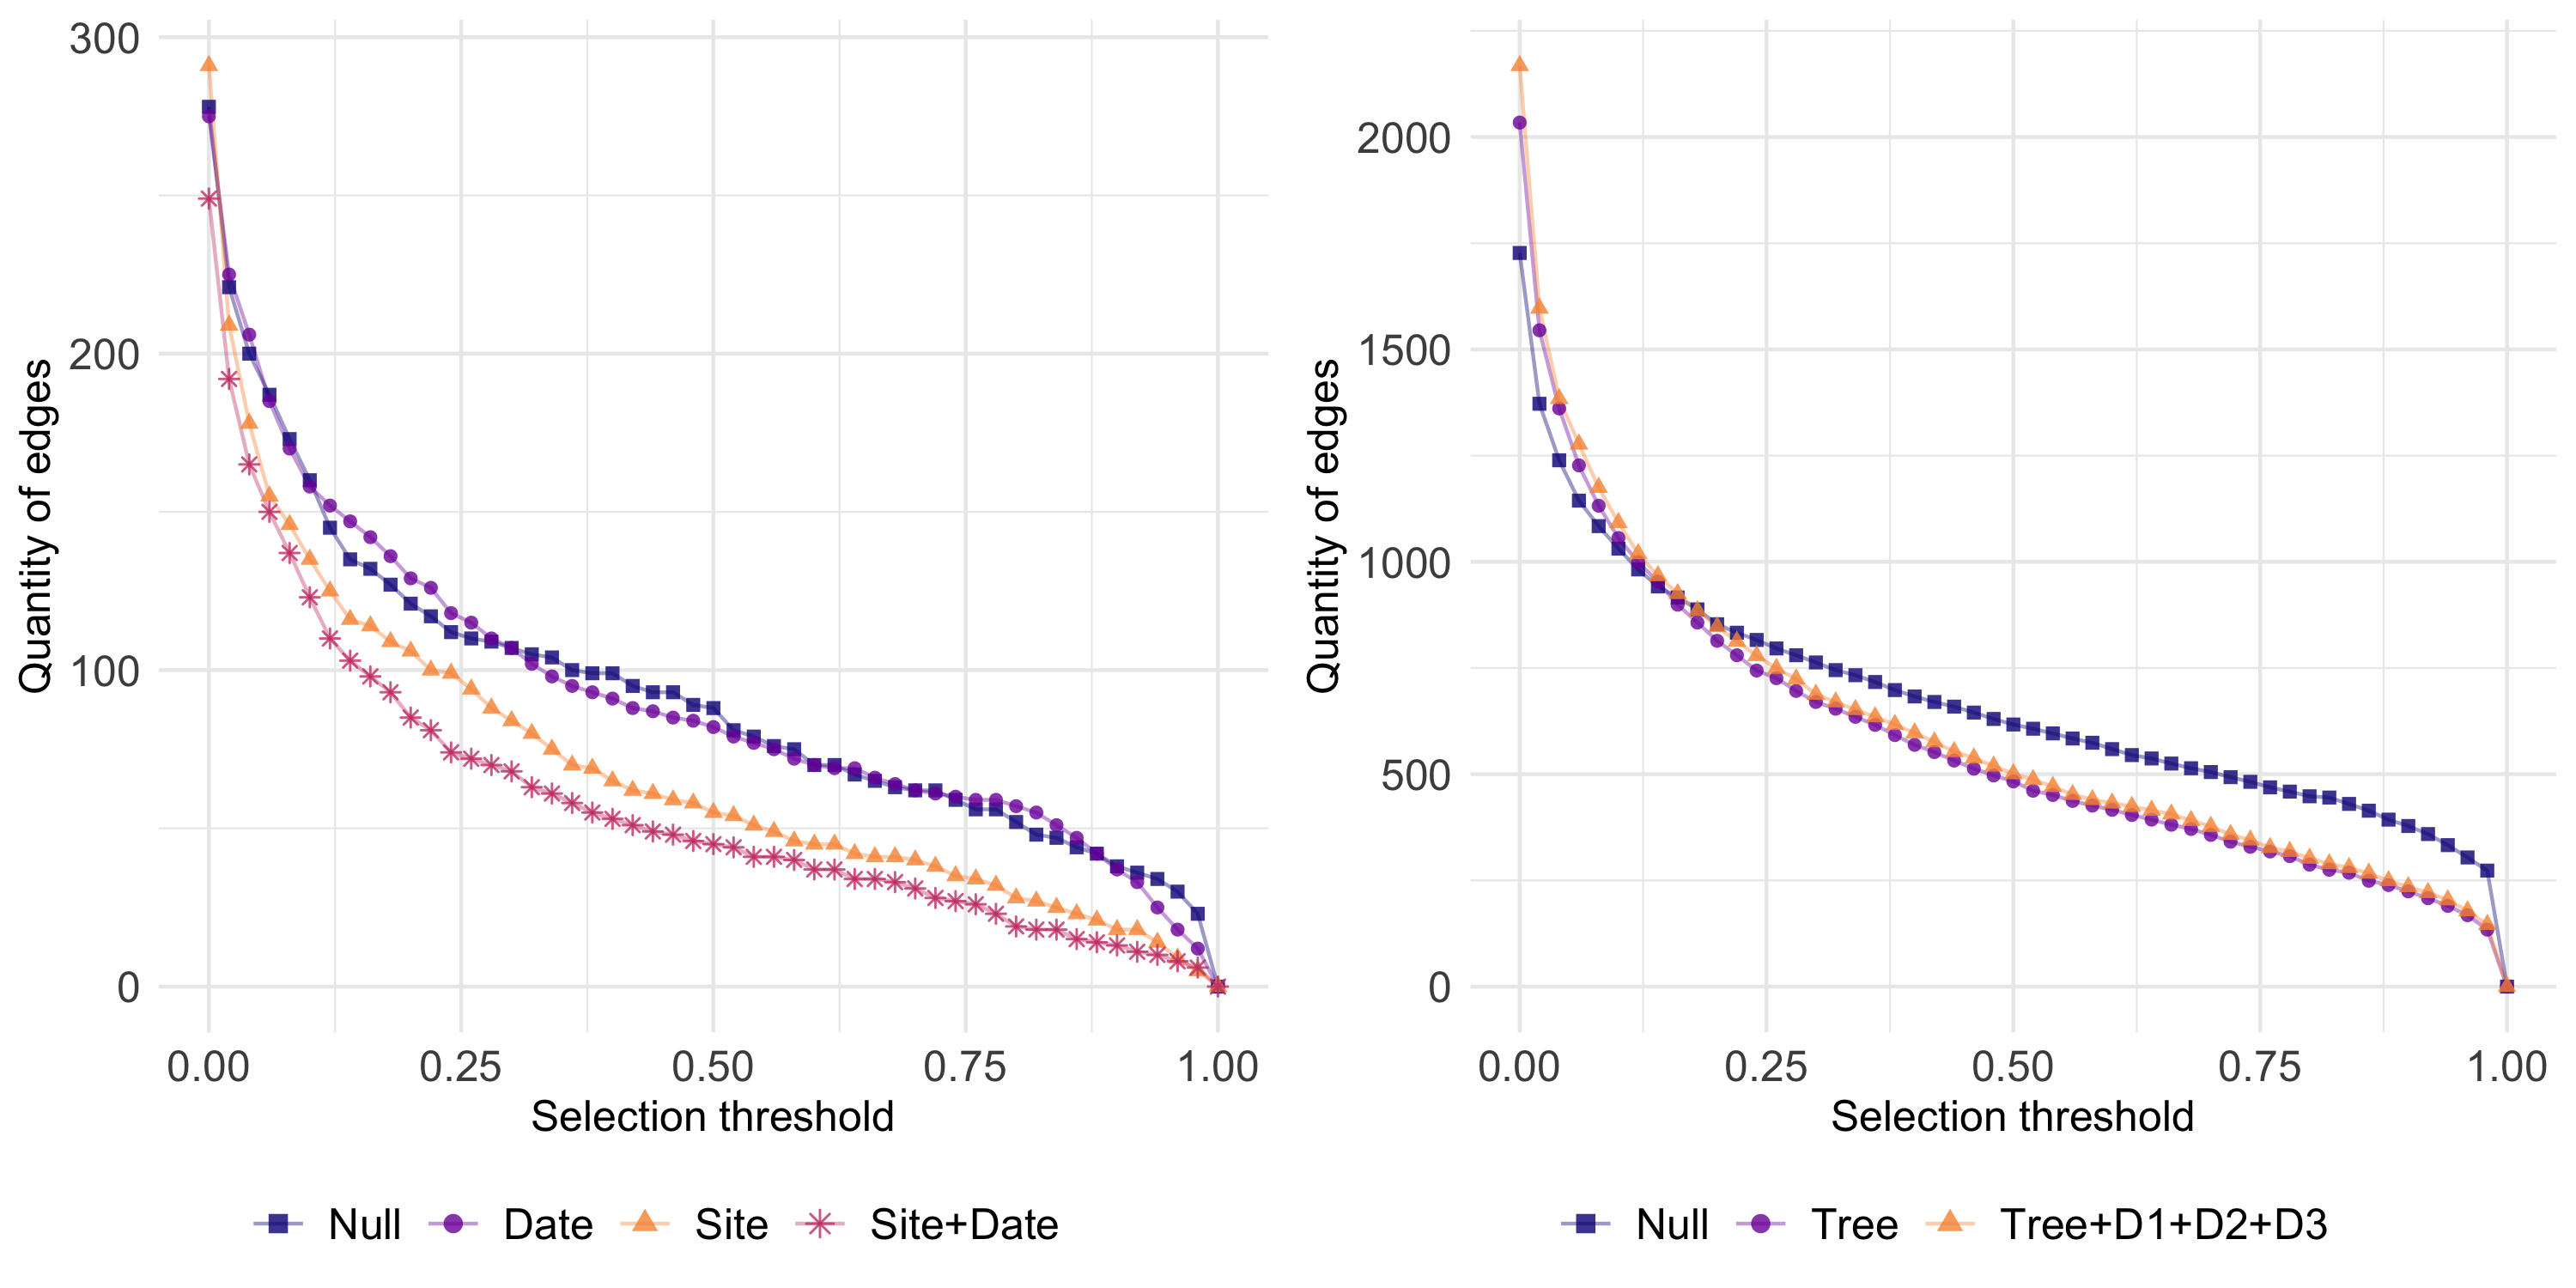
\includegraphics[width=\linewidth]{figs/QET_twoDataSets.png}
    \caption{Quantity of selected edges as a function of the selection threshold (\textit{left}: Fatala fishes, \textit{right}: oak mildew.)}
    \label{QETOak}
\end{figure}

The curves displayed on Fig. \ref{QETOak} are very smooth, which illustrates the difficulty of setting this threshold.


%\subsubsection{Illustrations: Fatala River fishes}
%\label{names_Baran}
%\paragraph{Species names with highest betweenness scores:}
%  13: Galeoides decadactylus; 19: Liza grandisquamis, 22:  Pseudotolithus brachygnatus, 25: Pellonula leonensis, 27:  Polydactylus quadrifilis, 30: Pseudotolithus typus, 32: Tylochromis intermedius.
